%!TEX root = ../BoYu-Dissertation.tex
\graphicspath{{Figures/}}

\chapter{Case Study: Promoting Awareness in Emergency Response} % (fold)
\label{cha:case_studies}

This chapter shows the feasibility and usefulness of the event-driven awareness promotion approach through a case study in the context of the emergency response. This case study aims to demonstrate the value of the event-driven awareness promotion approach in facilitating the emergency response operations by improved team awareness. The analysis of the case study consists in three steps:

\begin{enumerate}
	\item The first step of the case study is to gather knowledge about the current status of awareness support in emergency response operations.
	\item The second step includes the development of a concrete scenario, with the activities and events involved in the process. We describe the interaction between the activities and events, through which both the complexity and contingency scale up. On one hand is more events are generated as the activities are performed, and on the other hand is the increased number of adaptations that have to be made to the activities in order to address the problems caused by these events, such as resource assignment, top-down goal decomposition, and opportunistic re-planning.
	\item The third step consists of the analysis of several use cases of the EDAP system in the scenario developed in the preceding step. It focuses on demonstrating the key strengths of our approach, as it would be if EDAP platform was used to promote awareness in the scenario.
\end{enumerate}

\section{Awareness Support in Emergency Response} % (fold)
\label{sec:awareness_support_in_emergency_response}
Emergency is any natural or man-caused situation that results in or may result in substantial harm to the population or damage to property \cite{shen2004managing}. Emergency response is the collaborative activity of gathering resources and acting upon the problems immediately after an emergency happens. While the scope of emergencies can be very broad (e.g. biological, chemical, nuclear/radiological, incendiary, or terrorist), the emergency operations share some common characteristics that make them fit into the scope of collaborative activities discussed in this study:

\begin{enumerate}
	\item Emergency response is well recognized as a type of collaborative activities with a high level of complexity \cite{Turoff2004}. Emergency response usually involves multiple, distributed individuals and organizations to mitigate the impact of incidents that threaten public safety and the environment. During an emergency situation, workers rarely tackle tasks in an independent way. Instead, they find themselves working on a multitude of different activities, interleaving them in ways that seem best suited for getting their work accomplished given the practical pressures.
	\item Furthermore, exceptions to the planned responses are a common and critical factor in these activities. An unplanned-for contingency may have its genesis in numerous circumstances \cite{Mendonca2004}: an emergency situation may evolve, so that implemented plans are no longer applicable; it may be multi-faceted, requiring responding organizations to combine many plans in unexpected ways; and it may occur concurrently with other situations, thus creating resource shortages or outages.
\end{enumerate}

With the high level of complexity and contingency in emergency response operations, supporting awareness has been recognized as an important component of emergency response management (ERM) systems \cite{Turoff2004}. Situation awareness is a critical element of emergency decision making in a variety of operational contexts. Existing studies have shown that improved situation awareness can benefit operational effectiveness by facilitating the planning process \cite{Javed2011}, improving the quality and timeliness of decisions \cite{Blandford2004}, and offering better feedback on the appropriateness of actions arising from such decisions \cite{Chen2008}. With respect to supporting team-level awareness, research into and development of emergency response support has mainly focused on shared situation awareness \cite{Treurniet2012}, which has been considered as an essential prerequisite of an accurate collective picture of the emergency, and the basis of team decisions since they bring together and share individual perceptions, understandings, and predictions \cite{Javed2011}. However, the distributed nature of team-level awareness, i.e. the fact that awareness should be considered as a partly shared and a partly distributed understanding of a situation among team members, has not been well recognized and supported in existing emergency response management systems \cite{Treurniet2012}.

Current computational environments for awareness support in emergency response management favor the event-based awareness models for two reasons:

\begin{enumerate}
	\item The domain of emergency response has foundations in event driven task accomplishment \cite{Pottebaum2011}. Emergency response efforts are triggered by an incident, or a disaster, i.e. an ``event'' happening in the environment. To respond to the initial event, actors perform activities that add more events building up the situation. Decision makers have to react to these critical events for continuous response. Therefore the awareness they need is built up both from danger events as wells as emergency response events.
	\item Actors in the emergency response operations have to focus on information needed and the immediate situation factors that relate to the decisions and actions they are taking \cite{Turoff2004}. As a result, they have very limited attentional resources to actively monitor the environment and each other's work in order to pick up the awareness information peripherally. The event-based model has the advantage in pushing the information to the actors so that they do not need to switch their attentions to the periphery until the event are notified to them.
\end{enumerate}

Although much progress has been made to provide more effective event-based awareness support in emergency response operations with the integration of complex event-processing (CEP) engines (e.g. PRONTO \cite{Pottebaum2011} and PLAY projects \cite{Truptil2012}), the limitations of event-based models as we discussed in Section \ref{sec:the_state_of_art} also exist in the emergency response domain: 

\begin{enumerate}
	\item The effectiveness of event-based models largely depends on the quality of event subscriptions, which often requires considerable effort from the actors to explicitly manage. With the high level of complexity and contingency in emergency situations, existing event notification mechanisms either lead to too many irrelevant events notified to the actors, or the actors have to frequently modify subscriptions to adapt to their changing needs.
	\item The current event-based systems in the emergency response domain focus on the external events that are generated by physical sensors or complex events that are calculated by the rule-based event processing agent \cite{Pottebaum2011}, little support has been given to the social development of awareness, i.e. the internal events generated by the human actors.
\end{enumerate}

In the following of this Chapter, we describe a concrete emergency response scenario and then use it to argue how these limitations can be addressed in our event-driven awareness promotion approach.
% section awareness_support_in_emergency_response (end)

\section{An Emergency Response Scenario} % (fold)
\label{sec:an_emergency_response_scenario}
For this case study, we consider a nuclear crisis scenario in which a large quantity of radioactive substance is accidentally released in the atmosphere, due to a critical accident in a nuclear plant. The multiplicity and diversity of actors involved, the volume and heterogeneity of information, the critical dependencies between actions as well as the dynamics of the environment make the situation more complex. 

This scenario is based on the document analysis from several government websites, including the National Response Framework, the Nuclear/Radiological Incident Annex to NRF, NRC Incident Response Plan, as well as a collection of FEMA after action reports related to specific emergency exercise. To simplify the analysis, however, we reduce the complexity of the emergency response operations significantly in this scenario, comparing with the real world situations described in these documents.

\subsection{Overview of the scenario} % (fold)
\label{sub:overview_of_the_scenario}
\subsubsection{The field of work} % (fold)
\label{ssub:overview_of_the_field_of_work}
\paragraph*{Source of the incident} % (fold)
\label{par:source_of_the_incident}
The radiation leak in this scenario originates from the combination of two problems in a nuclear plan:
\begin{enumerate}
	\item Due to the wearing effect of time, a leak appeared in the steam generator. As a result, the water within the primary loop connecting the reactor and the steam generator, contaminated, spreads through the secondary loop.
	\item The throttle valve, a safety device of the secondary loop, opens due to the increased pressure inside the secondary loop. It does not respond to the manual bypass of the safety loop. As a result, the steam of the secondary loop, contaminated, escapes to the atmosphere.
\end{enumerate}
% paragraph source_of_the_incident (end)

\paragraph*{Actors} % (fold)
\label{par:actors}
To respond to the emergency caused by the radiation leak, many stakeholders are involved. The emergency operation center (EOC), in charge of operation, is formed with federal agencies, state and local public safety officials. Besides, firemen, policemen, and any other actors involved in the response process has one representative at the emergency operation center, to validate the feasibility of decisions, link with the field and ensure communication between actors. The EOC is distributed. Most of the decisions are made locally, where delegates are gathered, but decisions may also come from the national authority, state or local officials, or experts.

Besides the EOC, a large number of actors work in the filed to operate or support the nuclear crisis response. This includes (1) firemen to distribute iodine and rescue victims from the impacted area, (2) police to confine population and guide the evacuation, (3) decontamination and medical teams to assist victims, (4) transportation team to provide prompt delivery of personnel, equipment, and victims, (5) and scientific team to survey radiation, provide meteorologic information, and assess the evolution of the situation.
% paragraph actors (end)

\paragraph*{Resources} % (fold)
\label{par:resources}
A variety of resources are used by the actors in the scenario to perform their tasks. Some of the resources are used to perform specific tasks, such as the measuring equipment used by the scientific team to survey radiation, the medical equipment used by the decontamination and medical teams to assist victims. On the other hand, some of the resources are shared by multiple actions. The rescue vehicles can be used for transporting victims, delivering actors or other resources. The victims are manipulated by multiple actors in different tasks, such as decontamination, medical treatment, or transportation. The mobile decontamination or medical stations are used for operations on multiple victims. 
% paragraph resources (end)

\paragraph*{Actions} % (fold)
\label{par:actions}
The emergency response in the scenario is consisted of a large number of actions. We follow the analysis in \cite{Truptil2012} to structure the actions into three kinds of processes: decisional, operational and support process.

\begin{enumerate}
	\item The first process is dedicated to present the decisional part of the response operation. It concerns decision taking during the emergency response to plan and control the operational and support processes. These decisions help nuclear plant teams and public services to control nuclear repairing, to mobilize protection and relief resources, to communicate with media and local authorities and to animate the actual actions performed in the field.
	\item The operational process aims to resolve nuclear accident and its consequences. It concerns the actual actions performed in the field, such as protecting populations and rescue employees and populations. 
	\item The support process concerns the supporting actions dedicated to provide means to other processes. This consists of (1) making available resources and means and (2) assessing the situation continuously.
\end{enumerate}

Table \ref{tab:actions_in_scenario} shows a summary of the higher level structure of the actions. For each of these actions, subsidiary actions can be identified. These subsidiary actions can be further decomposed into more detailed actions. It is possible that each action can be decomposed in several ways following different plans. For example, the medical treatment on a victim can be performed by sending the victim to one of the medical stations and then treat the victim at the station, or if the victim is in an urgent situation, a medical team needs to be sent to the victim for immediate treatment.

{\footnotesize
	\begin{longtable}{>{\raggedright}p{0.8in}>{\raggedright}p{1.7in}>{\raggedright}p{2in}>{\raggedright}p{1in}}
\toprule 
\textbf{Type} & \textbf{Action} & \textbf{Subsidiary actions} & \textbf{Invovled actors}\tabularnewline
\midrule 
Decisional & To plan and control the operational and support processes & 1. To assign actors and relief resources

2. To communicate with media and local authorities 

3. To activate operational actions & Federal agency,

Local officials,

Delegates from different departments\tabularnewline
\midrule 
Operational & To protect population & 1. To alert/communicate

2. To confine population

3. To distribute iodine capsules

4. To evacuate population & Firemen, Police, Transportation team\tabularnewline
\midrule 
Operational & To rescue victims & 1. To search for victims

2. To decontaminate

3. To treat physical injuries

4. To transfer to new accommodation or hospital & Firemen, Decontamination team,

Medical team,

Transportation team\tabularnewline
\midrule 
Support & To support all reponse operations & 1. To deliver victims

2. To find and deliver equipment

3. To control traffic & Transportation team, 

Police\tabularnewline
\midrule 
Support & To assess situation & 1. To measure radioativity

2. To measure weather characteristics

3. To provide situational reports continuously & Scientific team\tabularnewline
\bottomrule
\caption{Actions in the nuclear emergency response scenario}
\label{tab:actions_in_scenario}
\end{longtable}
}
% paragraph actions (end)
% subsubsection overview_of_the_field_of_work (end)

\subsubsection{Events in the scenario} % (fold)
\label{ssub:events_in_the_scenario}
The demand for knowledge about events arises within the different processes in the scenario. Based on the sources where they come from, the events in the scenario can be clarified into five categories:

\begin{enumerate}
 	\item \emph{``Incident''} events represent actual or possible changes of the emergency incident. This type of events are generated by the scientific team during the action of assessing the emergency incident. Examples of these events include the changes to the measurements taken from the field, such as the change to the level of radiations, wind velocity and direction, as well as the results of analysis based on these measurements, such as the increased impacted area of the incident. 
 	\item \emph{``Risk''} events refer to the noticeable environmental changes that lead to (or potentially lead to) one or several risks on the emergency response operations. It may be linked to transportation risks as an accident or a traffic jam occurs. Or It may be the change of weather situations (e.g. raining) or fire/explosions risks that can complicate the response operations. 
 	\item \emph{``Resource''} events refer to the changes of resources, i.e. change of their availability in time and space, change of attribute values (e.g. quantity), or assignment to actions.
 	\item \emph{``Actor''} events refer to the changes of actors, such as the change of their locations, roles, or capabilities.
 	\item \emph{``Action''} events refer to the changes of actions, such as the changing execution state (e.g. the initiation, completion, or delaying of an action), the condition satisfaction, or the change of plan. 
 \end{enumerate} 

Table \ref{tab:events_in_scenario} lists some examples of the events in the scenario with relation to associated event types and possible event sources that produce them.

{\footnotesize
\begin{longtable}{>{\raggedright}p{1.8in}>{\raggedright}p{1.8in}>{\raggedright}p{1.8in}}
\toprule 
\textbf{Example Events} & \textbf{Event Type} & \textbf{Event Producer}\tabularnewline
\midrule 
\emph{Incident event}: Radioactivity level within 5 mile of the plant
exceeded 50 mSv/h & Vale comparison & Scientific team to measure radioativity\tabularnewline
\midrule 
\emph{Risk event}: A traffic jam occurs on the road between A and
B  & Existential change over time & Transportation team to deliver victims\tabularnewline
\midrule 
\emph{Actor event}: The army, who is not supposed to be involved in
iodine distribution, has to take part in the process & Conceptual relation & Officials to plan and control the operational actions\tabularnewline
\midrule 
\emph{Resources event}: Electricity generators will arrive at the
decontamination station in 1 hours... & Spatio-temporal relation & Transportation team to deliver the equipment\tabularnewline
\midrule 
\emph{Action event}: Iodine capsules have to be distributed to people
within 5 mile of the plan & Existential change over time & Officials to plan and control the operational actions\tabularnewline
\midrule 
Action event: New road signs have been placed to support the evacuation
plan & State change & Police to control traffic\tabularnewline
\bottomrule
\caption{Events in the nuclear emergency response scenario}
\label{tab:events_in_scenario}
\end{longtable}
}
% subsubsection events_in_the_scenario (end)
% subsection overview_of_the_scenario (end)


\subsection{Event-driven development of the field of work} % (fold)
\label{sub:event_driven_activity_development}
An important characteristic of the complex collaboration as this emergency response scenario is about to demonstrates is the interaction between the field of work and events. In the beginning, the aspects of the field of work in emergency response are changed by some initial events. Upon receiving these events, actors interpret them to assess the situation, then make decisions or perform actions that lead to more changes to the current field of work. These new changes can generate new events that trigger more changes to the filed of work. In this way, the collaborative activity is developed.

With the various entities in the field of work and the large number of events that can be generated in the scenario, it is a challenging task to describe the development of the whole emergency response process. To simplify the analysis of the scenario in the next section, we focus on the development of a sub-process of the scenario, i.e. the action to rescue victims from the impacted area. This sub-process itself is driven by a series of events and also generates new events. We consider several consecutive episodes in the process of rescuing a victim. Each of the episodes represents an example of a typical development trajectory of the collaborative activity that serves as the basic unit of analysis in this case study.

Table \ref{tab:development_trajectories} lists the four development trajectories that may happen in collaborative activities, and in the following of this section we describe the corresponding episodes representing them in the process of rescuing a victim. 

{\footnotesize
	\begin{longtable}{>{\raggedright}p{1.4in}>{\raggedright}p{2.5in}>{\raggedright}p{1in}}
\toprule 
\textbf{Trajectory Type} & \textbf{Description} & \textbf{Episode}\tabularnewline
\midrule 
Goal activation & A goal is activated by some triggering event, and then the action
to achieve the goal is developed through top-down decomposition & Episode 1\tabularnewline
\midrule 
Plan development & An event causes a new problem that is not addressed by the current
plan of an action. In order to the fix the problem the plan has to
be further developed. & Episode 2\tabularnewline
\midrule 
Responsibility transfer & An event leads to a breakdown in performing an action. To fix the problem, some actor has to perform an action that is out of the pre-defined responsibility. & Episode 3\tabularnewline
\midrule 
Opportunistic re-planning & An event leads to the decision that the current plan of an action
has to be abandoned and a new plan is developed. & Episode 4\tabularnewline
\bottomrule
\caption{Development trajectories in the field of work}
\label{tab:development_trajectories}
\end{longtable}
}

\subsubsection{Episode 1: Goal activation} % (fold)
\label{ssub:episode_1_goal_activation}
The first episode represents the initial development of the rescue action triggered by an event (Figure \ref{fig:episode_1_interaction}). 

\begin{figure}[htbp] %  figure placement: here, top, bottom, or page
   \centering
   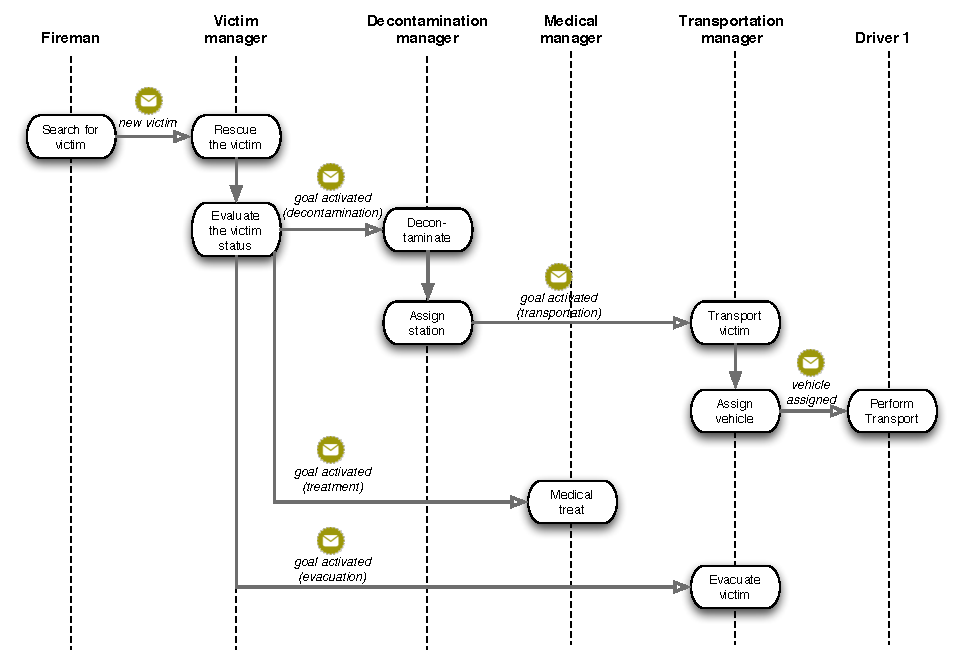
\includegraphics[width=5.8in]{episode_1_interaction.pdf} 
   \caption{Episode 1: Goal activation}
   \label{fig:episode_1_interaction}
\end{figure}

\begin{enumerate}
	\item It starts with the fireman's action to search for victims in the impacted area. When the fireman finds a new victim, she reports the discovery of the new victim as a new event.
	\item The event about the new victim is received by the victim manager ($VM$) and activates the $VM$'s goal that the victim needs to be rescued. The $VM$ decomposes the action to rescue the victim into sub-actions, and first evaluates the status of the victim. 
	\item Because the radiation level of the victim exceeds the threshold, the victim needs to be first decontaminated. As a result, the $VM$ generates a new event indicating the goal to decontaminate the victim is activated.
	\item Because the victim is also physically injured, the victim needs to be treated at a medical station after decontamination. As a result, the $VM$ generates another event indicating the goal to treat the victim is activated.
	\item After the treatment, the victim also needs to be evacuated to a shelter for recovery. The third event generated by the $VM$ describe the goal to evacuate the victim is activated.
	\item Upon receiving the event to activate decontamination, the decontamination manager $DM$ infers that the action to decontaminate is within her responsibility and she is capable of performing it, so she is committed to performing the action, decompose the action into sub-actions.
	\item To perform decontamination, $DM$ first needs to assign a decontamination station to the victim. After the assignment of station ($DS1$) to the victim, the $DM$ activates the goal to transport the victim to the station, which is described as a new event.
	\item Upon receiving the event that activates the goal to transport the victim to the station, the transportation manager $TM$ infers that the action to transport the victim to the station is within her responsibility and she is capable of performing it, so she is committed to performing the action, and further decompose the action.
	\item $TM$ first assigns a driver ($DR1$) with a rescue vehicle to the action, and an event describing the assignment of the driver ($DR1$) to the action to transport the victim is generated. Because the actual transportation action is out of the $DM$’s responsibility, she is waiting for the driver to perform it.
	\item Then the driver $DR1$ receives the event about the assignment and starts to perform the action.
	\item Besides, the medical manager $MM$ receives the event to activate the goal to treat the victim. However, because this action depends on the action to decontaminate the victim to be completed first, she has to wait for now.
\end{enumerate}

Episode 1 shows an example of how an initial event can trigger the actor to activate the goal to perform an action, and lead to top-down decomposition of the action. During the development of the action, more events are generated and more actors are participated into the action. The complete development trajectory of Episode 1 can be found in the Appendix (\ref{sec:episode_1_goal_activation}).
% subsubsection episode_1_goal_activation (end)

\subsubsection{Episode 2: Plan development} % (fold)
\label{ssub:episode_2_plan_development}
Episode 2 is built on top of Episode 1, showing how the current plan of the rescue action is further developed due to a problem caused by an event (Figure \ref{fig:episode_2_interaction}). 

\begin{figure}[htbp] %  figure placement: here, top, bottom, or page
   \centering
   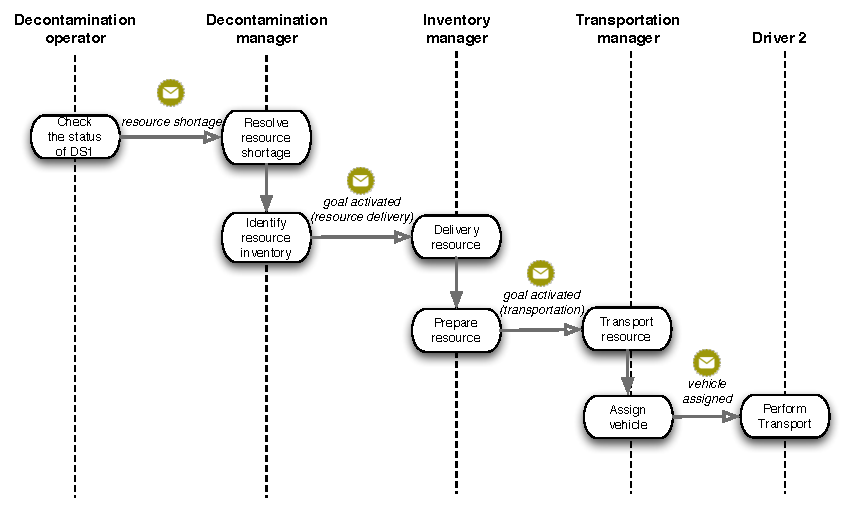
\includegraphics{episode_2_interaction.pdf} 
   \caption{Episode 2: Plan development}
   \label{fig:episode_2_interaction}
\end{figure}

\begin{enumerate}
	\item Episode 2 starts with an event that is reported by an operator at $DS1$, where the decontamination of the victim will be performed. The event shows that the quantity of an important resource, i.e. the available rinse tanks in $DS1$ is running low.
	\item The $DM$ receives this event and infers that the $DS1$ cannot work properly due to this resource shortage. In order to ensure the victim is successfully decontaminated, a new action to resolve the resource shortage needs to be added to the current plan of rescuing the victim.
	\item The $DM$ first needs to locate an inventory where the rinse tanks can be supplied. After identification of the inventory, the $DM$ activates the goal to deliver the resource from the inventory to the station, and a corresponding event is generated.
	\item Upon receiving the event about activating the goal to deliver the resource, the inventory manager $IM$ starts a new action to deliver the resource. The $IM$ first needs to prepare the resource for delivery. Once the resource is ready, she activates the goal to transport the resource to the station $DS1$, and the corresponding event is sent to the $TM$.
	\item Upon receiving the event, $TM$ starts a new action to transport the resource. $TM$ first needs to assign a driver $DR2$ with a rescue vehicle to the action, and an event describing the assignment of the driver ($DR2$) to the action to transport the resource is generated.
	\item Then the driver $DR2$ receives the event about the assignment and starts to perform the action.
\end{enumerate}

Episode 2 shows an example of the interleaving of planning and acting. Although this additional action (i.e. the action to resolve resource shortage) is not a required subsidiary component in the initial plan of performing the higher-level action (i.e. to rescue the victim), it is later added to the plan because of the problem of a resource is identified during the performance of the action. Details of Episode 2 is described in the Appendix (\ref{sec:episode_2_plan_development}).
% subsubsection episode_2_plan_development (end)

\subsubsection{Episode 3: Responsibility transfer} % (fold)
\label{ssub:episode_3_responsibility_transfer}
Episode 3 starts with an event leading to a breakdown in performing a subsidiary action, which can cause problem on the whole rescue action. To fix the problem, some actor has to perform an action that is out of her pre-defined responsibility (Figure \ref{fig:episode_3_interaction}).

\begin{figure}[htbp] %  figure placement: here, top, bottom, or page
   \centering
   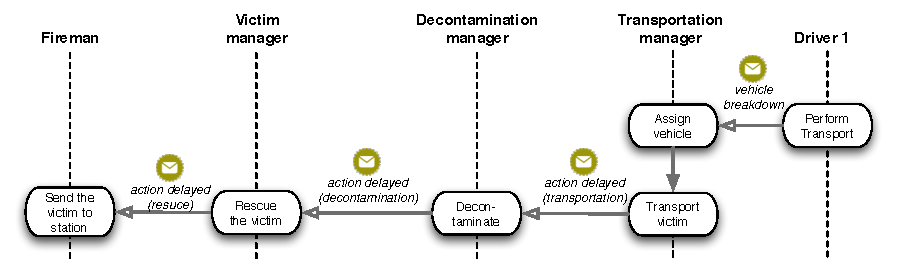
\includegraphics[width=5.8in]{episode_3_interaction.pdf} 
   \caption{Episode 3: Responsibility transfer}
   \label{fig:episode_3_interaction}
\end{figure}

\begin{enumerate}
	\item In the beginning of Episode 3, the rescue vehicle with the driver $DR1$ encounters a mechanical breakdown, as the driver is on the way to pick up the victim. The driver reports the problem as the initial event of Episode 3.
	\item The $TM$ receives the event and infers that because of the vehicle breakdown, the $DR1$’s action to transport the victim cannot be achieved. To solve the problem, the $TM$ attempts to assign another driver to perform the action. However, because all the drivers are currently in duty, the $TM$ cannot find a driver to perform the action until a later time. This problem is expressed as an event showing the action to transport the victim has to be delayed because of the unavailability of drivers.
	\item Upon receiving the event generated by $TM$, the $DM$ further infers that because of the delay to transport the victim, the action to decontaminate the victim will also be delayed, and a corresponding event is generated.
	\item Similarly, the $VM$ infers that because of the delay to transport the victim, the action to rescue the victim is delayed.
	\item The event generated by $VM$ is then received by the fireman who is with the victim in field. The fireman infers that although the delivery of the victim is not usually in the scope of her responsibility, she can help the rescue action by sending the victim directly to the decontamination station $DS1$. As a result, the fireman activates the goal to send the victim to $DS1$.
	\item Upon receiving the event from the fireman, $TM$ infers that because of the new action of the fireman, the responsibility of transporting the victim is now transferred from her to the fireman.
\end{enumerate}

Episode 3 demonstrates two important natures in the development of collaborative activities. First, it shows how the effect of one action can cascade to the other actions because of the dependencies among them. Second, it shows the transferability of actors' responsibilities in a complex collaboration. In order to achieve the shared goal of the group, the actors may have to undertake tasks that are not specified in their roles. Details of Episode 3 is described in the Appendix (\ref{sec:episode_3_responsibility_transfer}).
% subsubsection episode_3_responsibility_transfer (end)

\subsubsection{Episode 4: Opportunistic re-planning} % (fold)
\label{ssub:episode_4_opportunistic_re_planning}
The last episode shows the most significant change to the existing plan to rescue the victim. Because of the status change of the victim, the current plan to rescue the victim is no longer applicable and has to be replaced with a new plan (Figure \ref{fig:episode_4_interaction}).

\begin{figure}[htbp] %  figure placement: here, top, bottom, or page
   \centering
   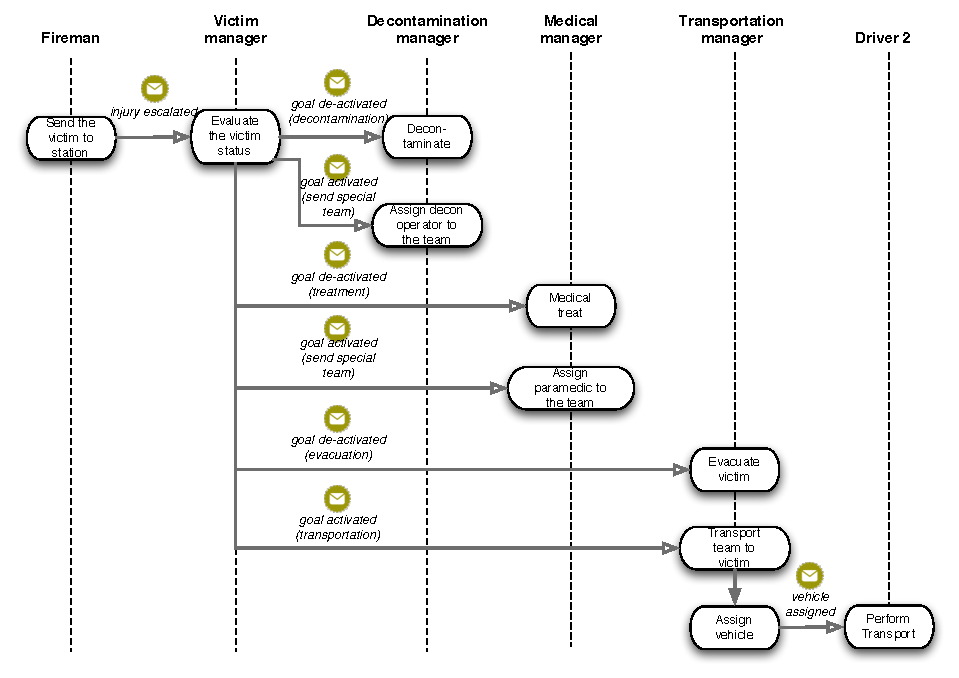
\includegraphics[width=5.8in]{episode_4_interaction.pdf} 
   \caption{Episode 4: Responsibility transfer}
   \label{fig:episode_4_interaction}
\end{figure}

\begin{enumerate}
	\item As the fireman decides to directly send the victim to the decontamination station, she finds that the physical injury of the victim becomes severe and prevents the fireman from moving the victim into the vehicle. The fireman has to report the status change of the victim as a new event.
	\item The event is received by the $VM$. $VM$ evaluates the situation of the victim and decides that because of the serious injury, the original plan to rescue the victim is no longer appropriate. A new plan needs to be adopted: a special team needs to be dispatched to the victim’s location to decontaminate and treat the victim on spot, and then the victim is directly sent to the hospital for further treatment. The changes to the plan are represented as a set of events and distributed to relevant actors.
	\item Upon receiving events from the $VM$, $DM$ first removes the current action to decontaminate the victim from her responsibility. Then $DM$ infers that in order to perform the action to dispatch a special team to the victim, a decontamination operator needs to be assigned to the team. By reviewing the available operators, DM decides on the operator who will be sent to the victim, and generate an event to indicate the assignment of the operator to the team.
	\item Similar to $DM$, the $MM$ first removes the action to treat the victim from her current responsibility, and decides on the medical professional that will be assigned to the special team. An event to indicate the assignment is then generated.
	\item The $TM$ removes the action to evacuate the victim from her current responsibility. Then the $TM$ infers that in order to perform the action to dispatch a special team to the victim, the action to transport the team to the victim needs to be activated. TM needs to assign a driver with a rescue vehicle to the action. Because the deactivation of the original decontamination action, the driver $DR2$ who was assigned for delivering the equipment during the decontamination action is now available for this action. As a result, $TM$ generates the event to describe the assignment of $DR2$ to the action to transport the special team to the victim.
	\item The driver $DR2$ receives the event about the new assignment and starts to perform the action.
\end{enumerate}

Episode 4 shows how one action can be performed using different plans in different situations. Triggered by the initial event, the action has to be opportunistically re-planned to adapt to the changing environment. In the re-planning process, the resources that are bound to the old plan are released and can be assigned to other actions in the new plan. For example, the rescue vehicle with the driver $DR2$ was assigned to perform the resource delivery action, however after the re-planning, it is now re-assigned to a new action to deliver the rescue team (Details of Episode 4 is described in Appendix (\ref{sec:episode_4_opportunistic_re_planning})). 

% subsubsection episode_4_opportunistic_re_planning (end)
\subsubsection{Discussion} % (fold)
\label{ssub:discussion}
The four episodes demonstrates several characteristics of the collaborative activity in the emergency response scenario:

\begin{enumerate}
	\item From the four episodes, we can see how the complexity of the collaborative activity is coupled with the different types of contingency. In the beginning, the activity can be quite simple, with limited actors involved and standard work flow. However, due to the various exceptions that may occur in the process, much more effort is given to fix the problems and breakdowns in the collaborative activity. As a result, more actors are involved into the field of work, and the plan of the activity has to be modified significantly. The coupling of complexity and contingency makes the actors' awareness need become unpredictable in the beginning of the collaborative activity.
	\item These episodes show good examples of the interaction between events and field of work. On one hand is the events triggering the development of the field of work, and on the other hand is the changes to the field of work generate new events. It is within this recursive cycle between the events and the field of work that the knowledge about the collaborative activity is built up. This provides the basic for our approach and in next section, we will demonstrate how the knowledge updating process in our approach works in this scenario. 
	\item These episodes also illustrate the social development of awareness across multiple actors. Along with the development of the activity is how the events are generated by different actors to express their interpretation of the situation, and then are consumed by other actors. In Section \ref{sec:promoting_awareness_in_the_scenario}, we will demonstrate how the social development of awareness in these episodes can be supported in our approach.
\end{enumerate}
% subsubsection discussion (end)
% subsection event_driven_activity_development (end)
% section an_emergency_response_scenario (end)

\section{Knowledge representation and updating in the scenario} % (fold)
\label{sec:knowledge_representation_and_updating_in_the_scenario}

% section knowledge_representation_and_updating_in_the_scenario (end)

\section{Promoting awareness in the scenario} % (fold)
\label{sec:promoting_awareness_in_the_scenario}

% section promoting_awareness_in_the_scenario (end)

Possible variables:

1. complexity of interdependencies (e.g. the number of dependencies)

2. task-specific asymmetries (e.g. to what extent the local scopes are overlapped)
 
3. dynamics (e.g. chances of re-planning)

4. concurrent multiple activities

Demonstrate three features:

1. The effectiveness of using local scope to reduce complexity:

As the field of work grows, the local scope stays relatively stable

Strategy: generate the PlanGraph model in three different application domains, showing how complex the PlanGraph model can become, but at the same time the local scope for each actor is relatively small.

2. The effectiveness of using local scope to manage subscription, especially for handling dynamics

Strategy: (1) define an actor's information needs; (2) use the content-based approach to generate the set of subscriptions; (3) use our local-scope approach to generate the set of subscriptions; (4) compare the number of subscriptions that the user needs to generate in each case; (5) make changes to the activity model, compare the number of modifications needed for both approaches.

3. Show how could the social event chain be used in the coordination work? Some possibilities:

(1) the ability to detect conflicts/duplicates

(2) the ability to seek/offer help



\section{Activity-Based Approach} % (fold)
\label{sec:activity_based_approach}
\subsection{Types of Events} % (fold)
\label{sub:types_of_events}
\subsubsection{External and internal events} % (fold)
\label{ssub:external_and_internal_events}
To understand events in geo-collaboration, an important distinction has to be made between \emph{external} events (in the environment) and internal events (in the activities). 

External events are changes in the physical environment that have impact on the performance of collaborative activities. For instance, the occurrence of a traffic accident may block the traffic flow, which makes an actor’s activity of delivering equipment to a medical station impossible to finish on time. External events in the environment can be characterized in three major categories: changes of identity (e.g. the occurrence of a traffic accident), attribute changes of an object (e.g. the contamination level of the chemical plan is increased), or spatial changes (e.g. the impacted area is enlarged due to the wind condition).

Internal events are state changes on the basic elements (i.e. resources, goals, activities) of geo-collaboration. Resource events indicate changes on the state of any resources that are used in the activities. Resource events can impact response activities in different ways: (1) the creation of a new resource can trigger new activities (for example, a new victim may lead to the activity to perform decontamination and medical treatment); (2) the state change of a resource can impact the activity that requires the use of the resource (e.g. the mechanical breakdown of a vehicle makes the delivery activity unable to complete); (3) the state change of a resource can enable/disable the activity that depends on it (e.g. a victim’s location change leads to the satisfaction of a precondition that the victim must be located at the medical station, which further enables the activity to perform medical treatment on the victim). Condition events indicate changes on a certain relationship between multiple objects in a collaborative activity. For example, a condition may express a spatial relationship that the victim must be located at the decontamination station. The condition will change the state from open to holding when a driver has picked up the victim and transpored him/her to the station. Activity events are described as change of activity states, such as the initiation of a new activity, the completion or delay of an ongoing activity. 

The distinction between external and internal events is very important to identify the set of events that should be captured and modeled in the awareness mechanism. Not all the external events in the environment are important for the actors to perform their activities. Rather, only a subset of the external events that can lead to changes within the activities (i.e. the internal events) is meaningful. The derivation of internal events from external events is an active cognitive process that requires interpreting the meaning of external events within the context of the collaborative activities.
% subsubsection external_and_internal_events (end)

\subsubsection{Local and remote events} % (fold)
\label{ssub:local_and_remote_events}
The distinction between external and internal events is based on the boundary between the surrounding environment and the overall collaborative activities as a whole. However, in order to understand the awareness information needed for each individual, another important distinction between local and remote events has to be made. 

The local and remote events are defined with aspect to the local scope of work for each individual actor. Local events reflect the state changes of basic elements (i.e. resources, goals, activities) within an actor’s local scope of work. For instance, the report of a new victim that needs to be decontaminated, the exceeding capacity of a decontamination station are local events within the decontamination manager’s local scope of work. Remote events are the changes outside an actor’s local scope of work. For instance, a victim that doesn’t need to be decontaminated is transported to a shelter is a remote event for the decontamination manager. The distinction of local and remote events is relative to each individual actor. A local event of one actor may be a remote event for another actor due to their different local scopes of work. In addition, a remote event can be internal, reflecting the state changes of another actor’s activities, or it can be external, reflecting changes in the environment. 

The distinction between local and remote events is important to identify the relevance of events that should be notified to each actor. Local events reflect changes within an actor’s local scope of work and therefore are directly relevant to the actor. On the other hand, due to the existence of the web of dependencies among activities, some of the remote events can (or potentially can) lead to changes in the actor’s local scope of work, i.e. the impact of a remote event may be propagated to the local scope of the actor as derived local events, and therefore they also become relevant. For instance, the traffic jam on the road is a remote event for the decontamination manager. However, because the traffic jam happens on the way of a victim to be delivered to a decontamination station, it can potentially delay the decontamination operation on the victim, which becomes a relevant local event for the decontamination manager. As a result, the goal of an awareness system is to notify an actor not only all the relevant local events, but also the subset of remote events that can be propagated to the actor’s local scope through the web of dependencies. 

% subsubsection local_and_remote_events (end)
% subsection types_of_events (end)

\subsection{Event Subscription} % (fold)
\label{sub:event_subscription}
\subsubsection{Specifying Local Scopes} % (fold)
\label{ssub:specifying_local_scopes}

% subsubsection specifying_local_scopes (end)

\subsubsection{Defining Event Patterns} % (fold)
\label{ssub:defining_event_patterns}

% subsubsection defining_event_patterns (end)
% subsection event_subscription (end)

\subsection{Event Matching} % (fold)
\label{sub:event_matching}

% subsection event_matching (end)

% section activity_based_approach (end)

\section{A Simulation Experiment} % (fold)
\label{sec:a_simulation_experiment}
We conduct a simulation experiment to compare the content-based event notification approach and the proposed activity-based approach. The basic hypothesis is that, in dynamic environment where the user's activity changes frequently, the proposed activity-based approach provides a more accurate way for the user to express their awareness interests than the content-based approach. We use the emergency response scenario as described in the Introduction Chapter to perform the experiment, from the perspective of the decontamination manager.

\subsection{Variables of Interests} % (fold)
\label{sub:variables_of_interests}
We are interested in the capability of these two notification approaches in handling different types of activity dynamics. Particularly, we are interested in three types of dynamics that may occur in the scenario: 
\begin{enumerate}
	\item \textbf{Parameter Change}: the value of a parameter is changed. In the scenario, it can be the case when the decontamination manager re-assign a new station where a victim will be decontaminated.
	\item \textbf{Plan Development}: the plan of the actor is changed. In the scenario, it can be the case when the decontamination manager starts to concern about certain equipment delivery after the stock is running low.
	\item \textbf{Local Scope Change}: the actor's local scope of work is changed. In the scenario, it can be the case when another manager joins the activity, and take a subset of tasks away from the modeling manager.  
\end{enumerate}

To perform the experiment, we define four scenes to reflect the three types of activity dynamics:
\begin{enumerate}
	\item Initial scene ($S_0$): indicates the current state of the decontamination manager's activities
	\item Parameter change scene ($S_1$): indicates one of the parameters of the decontamination manager (station) has been assigned with a new value, comparing with $S_0$
	\item Plan development scene ($S_2$): indicates one of the conditions has been elaborated into a more concrete plan, comparing with $S_1$
	\item local scope change ($S_3$): indicates the another actor joins the activity, and the local scope of the modeled user has been reduced to a smaller set, comparing with $S_2$
\end{enumerate}
% subsection variables_of_interests (end)

\subsection{Simulating Event Generation} % (fold)
\label{sub:event_generation}
A set of events are randomly generated based on the whole group activities. Given the current PlanGraph model, the events can happen on any of the activity, resource, or condition node, and indicate any types of possible changes that are defined in Chapter 5.
% subsection event_generation (end)

\subsection{Creating Subscriptions} % (fold)
\label{sub:content_based_subscriptions}
Two sets of content-based subscriptions will be generated. 
\begin{enumerate}
	\item The first set of subscriptions are defined merely based on the current interest of the manager in the initial scene ($S_0$). This set only includes the events that are relevant to the manager's current activities. Therefore, it can be considered as the minimal subscription set of events, using the content-based notification approach ($CON_{min}$).
	\item The second set of subscriptions are defined based on considering all the three possible activities dynamics defined in scenes ($S_1$, $S_2$, $S_3$). It includes all the possible events that might be relevant to the manager in all the scenes. Because we attempt to include the maximum set of events that could be relevant for the manager across all the scenes, we define this content-based subscription as ($CON_{max}$).  
\end{enumerate}

In addition, the activity-based subscription will also be generated, following the steps described in previous section. The subscription includes the specification of local scope of the decontamination manager, his/her intentions and detailed event patterns on each node in the local scope. We define this activity-based subscription as $ACT$.
% subsection creating_subscriptions (end)

\subsection{Procedures} % (fold)
\label{sub:procedures}
The experiment includes four runs. 
\begin{enumerate}
	\item The first run $R_0$ is the human judgment on the relevance of the simulated event set to form the baseline result. The human analysts run through the list of simulated event set to decide on whether each event is relevant to the modeled decontamination manager, under the four scenes respectively. To reduce the subjective errors of human judgment, two analysts will perform the judgment separately and then discuss on the differences to form the final sets of events.
	\item In the second run $R_1$, the simulated event set will be fed into the matching program following  content-based notification approach, using the set of subscriptions defined as $CON_{min}$.
	\item In the third run $R_2$, the simulated event set will be fed into the matching program following  content-based notification approach, using the set of subscriptions defined as $CON_{max}$.
	\item In the fourth run $R_3$, the the simuated event set will be fed into the matching program following activity-based notification approach, using the set of subscriptions defined as $ACT$.
\end{enumerate}
% subsection procedures (end)

\subsection{Measures} % (fold)
\label{sub:measures}
Two measures will be used to compare the results of different notification approaches:
\begin{enumerate}
	\item \textbf{Miss rate} is defined as the ratio between number of events that are considered as relevant in $R_0$ but missing in the result of $R_i$ ($i \in \{1, 2, 3\}$), and the total number of events considered as relevant in $R_0$.
	\item \textbf{False alarm rate} is defined as the ratio between number of events that are considered as relevant in $R_i$ ($i \in \{1, 2, 3\}$), but missing in the result of $R_0$, and the total number of events considered as relevant in $R_i$ ($i \in \{1, 2, 3\}$).
\end{enumerate}

% subsection measures (end)

\subsection{Results} % (fold)
\label{sub:results}
Some results we expect from the experiment can be:

\begin{enumerate}
	\item Comparing with the context-based notification using subscriptions defined as $CON_{min}$, the activity-based notification has lower miss rate in the scenes $S_1$, $S_2$, $S_3$. The difference between miss rates of the two methods increases as the scene evolves.
	\item Comparing with the context-based notification using subscriptions defined as $CON_{max}$, the activity-based notification has lower false alarm rate in the scenes $S_1$, $S_2$, $S_3$. The difference between false alarm rates of the two methods decreases as the scene evolves.
\end{enumerate}

% subsection results (end)

\subsection{Discussion} % (fold)
\label{sub:discussion}

% subsection discussion (end)


% section a_simulation_experiment (end)
\section{The Cognitive Basic} % (fold)
\label{sec:the_cognitive_basic}
The cognitive principles that guide the design of visual displays for event interpretation.

\begin{enumerate}
	\item The schemata theory (Bartlett et al.): when human respond to incoming stimuli, they make use of their existing knowledge as a frame of reference to make sense of the incoming stimuli and produce behavior. The active organization of existing knowledge is defined as `schema'. Schemata can be merely mental templates in human mind, or retrieved dynamically from the external visual artifacts. 
	\item The relevance principle (Kosslyn 2006): Visual displays should present no more or no less information than is needed by the user. Presenting all of the relevant information in the display relieves the user of the need to maintain a detailed representation of this information in working memory, where presenting too much information in the display leads to visual clutter or distraction by irrelevant information (Rosenholtz et al. 2007; Wickens \& Carswell, 1995).
	\item The task specificity principle (Hegarty et al. 2009). Visual displays are used for many different tasks, and there is no such thing as a `best' visual display, independent of the task to be carried out with this display. 
\end{enumerate}

What these cognitive principles can inform us are:
\begin{enumerate}
	\item When the user interprets an awareness event, he/she needs to activate and connect the event to his/her contextual knowledge of the situation. The visual display can enhance the interpretation by externalizing part of the knowledge in the visual representation and freeing up working memory resources.
	\item However, the effectiveness of the visual display depends on how much relevant information is represented. We want to provide the users with just enough contextual information without causing visual clutter or distraction.
	\item The relevance of contextual information to be displayed is dependent on the current task to be carried out, or the decision that need to be made by the user.

\end{enumerate}
% section the_cognitive_basic (end)

\section{Activity-Aware Event Interpretation} % (fold)
\label{sec:activity_aware_event_interpretation}
The problem we want to address here is that: how the computational model of activities and local scopes can inform the system to decide on what contextual information should be displayed when the users interpret awareness events.

The decisions can be made based on two factors: the incoming event and the activities/local scope the user is working on. By maintaining the PlanGraph model, the system can infer how the event will impact the user's activities, which can be used to infer what decisions the user needs to make next, or what tasks the user will focus on, which can be used to decide on what should be displayed on the user interface.

Generate the set of rules based on SharedPlan Theory.

Some examples:

1. If the event initiates a new goal of the user, by elaborating on the plan, the system can infer that the user will work on identifying the set of parameters first.

2. If the event indicates the failure of a parameter, and there is no plan to fix the failure, the system can infer that the user will re-assign the values of this parameter.

3. if the event indicates the failure of a parameter, and there is plan to fix the failure, the system can infer that the user will work on the plan to fix it.

% section activity_aware_event_interpretation (end)

\section{Experimental Study}
\subsection{Hypotheses} % (fold)
\label{sec:hypotheses}
The general assumption is that maps with contextual information that is adapted to the user's current activities are more effective to support awareness event interpretation, than maps with fixed contextual information.
% section hypotheses (end)

\subsection{Experimental Design} % (fold)
\label{sec:experimental_design}
\subsubsection{Participants} % (fold)
\label{sub:participants}
Twelve undergraduate or graduate students will be recruited as participants in this study. All participants need to use computers on a daily basis. Prior experience with emergency response planning or operations is welcomed, but not required.

% subsection participants (end)
\subsubsection{Tasks} % (fold)
\label{sub:tasks}
The participants are asked to perform simulation tasks in an emergency response scenario, from the perspective of the decontamination manager. The tasks that the participants need to perform are driven by the events they receive.

Some example events and triggered tasks include:

\begin{enumerate}
	\item E1: A new victim that needs to be decontaminated is reported by the victim manager. The task that the participant needs to do is to assign a decon station for the victim.
	\item E2: The impacted area is enlarged and a decon station becomes inside of the impacted area. The task that the participants need to do is to re-assign the victims that are assigned to the station to other stations.
	\item E3: A type of resource in a particular decon station is running low in stock. The participant need to request for a resource delivery from one of the suppliers.
	\item E4: The delay on a victim's arrival at assigned station. The participant needs to check whether it will conflict with the victim's deadline on decontamination. If so, he/she needs to plan for sending the victim to other station.
\end{enumerate}

% subsection task (end)

\subsubsection{Design settings} % (fold)
\label{sub:design_settings}
Participants are randomly assigned to one of the two design settings in one experiment session to perform their tasks. The three design settings are described as follow: 
\begin{itemize}
    \item The first design setting ($D_1$) shows a map showing locations of all the stations, victims, and resource suppliers as separate layers. The user can turn on/off each layer, or filter the objects based on spatial distances.
    
    \item In the second design setting ($D_2$), the features displayed in the map are adapted based on the event and the tasks that the user needs to perform. 
\end{itemize}
% subsection design_settings (end)

\subsubsection{Procedure} % (fold)
\label{sub:procedure}
In the beginning of each experiment session, the participant is randomly assigned to one of the three design settings and given a couple of minutes to learn the functions of the assigned design setting. In addition to the training of the simulation system, the participant is also provided with the general picture of the collaborative activity. Information about other agents, related resources in the activity, and the current goals and tasks of the group are presented to the participant, so he/she has a clear understanding of the task in the context of the whole activity and provides the basis for interpreting the awareness events. After the training session, the participant is asked to perform the simulation task. During the performance of the task, the participant is notified with a list of awareness events, and asked to finish the assessment form to answer relevant questions after each event notification.

Each experiment session is composed as a series of interaction episodes between the participant and the system. Each interaction episode defines how an agent (role-played by the participant) responds to a particular event in the collaborative scenario. Each interaction episode starts with the provision of an awareness event in the interface, and then the participant is perform corresponding tasks based on their understanding of the event.

% subsection procedure (end)

\subsubsection{Measurement} % (fold)
\label{sub:data_collection}
To measure the overall performance during the experiment session, we record the completion time of each experiment session and the participant's responses to each awareness event. In the design phase of the awareness events, each event is associated with a set of optimal responses. The participant's responses are then compared with the optimal set to indicate the quality level of task completion. 

% section data_collection (end)

\subsection{Results} % (fold)
\label{sec:results_and_discussion}
In general, we expect that 

1. the participants in design setting $D_2$ will generate more valid responses than the participants in design setting $D_1$.

2. the participants in design setting $D_2$ should spend less time to finish the tasks than the participants in design settings $D_1$ in average.
% section results_and_discussion (end)

\subsection{Discussion}

% chapter case_studies (end)




 

